\documentclass[12pt]{article}

\title{Fractal dimension in the simulation of the non-relativistic gravitation of disk-like zero pressure density systems}
\author{S. Halayka\footnote{sjhalayka@gmail.com}}
\date{\today\;\currenttime}

\usepackage{datetime}
\usepackage{listings}
\usepackage{cite}
\usepackage{xcolor}
\usepackage{graphicx}
\usepackage{setspace}
\usepackage{amsmath}
\usepackage{url}
\usepackage[margin=0.8in]{geometry}
\usepackage{listings}


\usepackage{xcolor}
\lstset { %
    language=C++,
    backgroundcolor=\color{black!5}, % set backgroundcolor
    basicstyle=\footnotesize,% basic font setting
    showstringspaces=false,
}


%\doublespace

%\usepackage[]{lineno}
%\linenumbers


\begin{document}



 
\maketitle

\begin{abstract}
Solutions for Newtonian (e.g. Keplerian) and Galactic flat rotation curve gravitation are given in terms of gravitational field lines.
C++ code is provided.
\end{abstract}



\section{Introduction}

At first, we define entropy in terms of the $n$-bit integers.

Then we discuss the brute force numerical solution of the equations for the Newtonian (e.g., Keplerian) orbit, and the Galactic flat rotation curve orbit.

Next, we use a heuristic, analytical approach to the solve the equations for the Galactic flat rotation curve orbit.

Finally, we visualize the difference between the Newtonian (e.g., Keplerian) orbit and the Galactic flat rotation curve orbit, in terms of the relativistic Doppler effect.

In this paper, we consider that the pressure density is near zero at the Galactic scale (e.g. at interstellar distances, there is no pressure acting between the stars), which simplifies the equations, and allows for anistropic gravitation in the first place.



\section{Entropy}
Entropy is a measure of how much information is required to encode a set of microscopic states (e.g. microstates).
Where there are $W$ distinct microstates, the Shannon binary entropy $n$ is:
\begin{equation}
n =  \frac{-\sum_{i = 1}^{W} p_i \log p_i} {\log 2},
\end{equation}
where $p_i$ is the probability of the $i$th microstate, and all probabilities add up to $1$:
\begin{equation}
\sum_{i = 1}^{W} p_i = 1.
\end{equation}
For equiprobable microstates, like in the case of the 8-bit integers for instance, where $p_i = 1/W$, the equation for $n$ greatly simplifies:
\begin{equation}
n = \frac{\log W}{\log 2}.
\end{equation}
The number of equiprobable, distinct 8-bit integers is $2^8 = 256$, and so $n = 8$ and $W= 256$.
This is to say that if you understand the concept of the 8-bit integers, then you also understand binary entropy in the case of equiprobable microstates.
For the 16-bit integers, $n = 16$ and $W = 65536$, and so on and so forth.

At low density (e.g. everyday densities on the Earth), this binary entropy is proportional to mass.
The Boltzmann binary entropy is:
\begin{equation}
n = \frac{k \log W}{\log 2}.
\end{equation}

At the highest density (e.g. black hole densities), this binary entropy is proportional to mass squared.
The Bekenstein-Hawking binary entropy is:
\begin{equation}
n = \frac{A_s k c^3}{ 4 G \hbar \log 2}.
\end{equation}

The following is a code for calculating the entropy of a string of characters.
Note that the calculation allows for non-equiprobabilities, and so it's a bit more general.
\begin{lstlisting}
#include <iostream>
#include <map>
#include <string>
#include <sstream>
#include <cmath>
using namespace std;

int main(void)
{
    // Non-equiprobable
    string input_string = "Hello world";

    // Equiprobable
    //string input_string = "abcdefgh";

    size_t length = input_string.length();

    ostringstream output_stream;
    
    double entropy = 0.0;
    
    if(length > 0)
    {
        map<char, size_t> input_map;

        for(size_t i = 0; i < length; i++)
            input_map[input_string[i]]++;
        
        for(map<char, size_t>::const_iterator ci = input_map.begin(); 
			ci != input_map.end(); 
			ci++)
        {
            double probability = ci->second / static_cast<double>(length);
            
            output_stream << 
			"Character: \'" << ci->first << 
			"\', Count: " << ci->second << 
			", Probability: " << probability << 
			endl;
            
            entropy += probability * log(probability);
        }
        
        entropy = -entropy / log(2.0);
    }

    cout << output_stream.str() << endl;
    cout << "Entropy: " << entropy << endl;
    
    return 0;
}

\end{lstlisting}




\section{Brute force: field line intersection density gradient}

It was Gerard 't Hooft's idea to quantize the black hole's event horizon area into gravitational field line emitters (e.g. dividing the entropy by $\log 2$) in his pioneering work on the holographic principle.

In this paper we numerically solve for the Newtonian (e.g. Keplerian) and flat (e.g. constant velocity) gradients (e.g. derivatives) using an axis-aligned bounding box by obtaining the lengths of the intersecting field line segments emitted by the gravitating body. See Fig.1. 

Here, 
\begin{equation}
D = (2, 3]
\end{equation}
stands for dimension, and 
\begin{equation}
d = 3 - D = [0, 1)
\end{equation}
stands for disk-like.

Regarding the holographic principle, the Schwarzschild black hole event horizon radius is:
\begin{equation}
r_s = \sqrt{\frac{A_s}{4 \pi}} = \sqrt{\frac{n G \hbar \log 2}{k c^3 \pi}},
\end{equation}
and the mass is:
\begin{equation}
M = \frac{c^2 r_s}{2 G} = \sqrt{\frac{n c \hbar \log 2}{4 G k \pi}}. 
\end{equation}

Where $R$ is some far distance from the centre of the gravitating body (e.g, $R \gg r_s$), $\beta$ is the get intersecting line length density function, and $\epsilon$ is some small value (e.g $10^{-5}$), the gradient is:
\begin{equation}
\gamma = \frac{\beta(R + \epsilon) - \beta(R)}{\epsilon}.
\end{equation}
The following equation for the gradient strength was found to be true through trial and error:
\begin{equation}
g = -\gamma \pi = \frac{n}{2 R^D}.
\end{equation}
Thus, the Newtonian acceleration $a_{\textit{Newton}}$, where $D = 3$, is:
\begin{equation}
a_{\textit{Newton}} = \frac{v_{\textit{Newton}}^2}{R} = \sqrt{\frac{n G c \hbar \log 2}{4 k \pi R^4}} = \frac{GM}{R^2},
\end{equation}
and the acceleration $a_{\textit{flat}}$ for a flat rotation curve, where $D < 3$, and $v_{\textit{flat}}$ is known via observation of the relativistic Doppler effect, is:
\begin{equation}
a_{\textit{flat}} = \frac{v_{\textit{flat}}^2}{R}.
\end{equation}

The ratio of the two accelerations is:
\begin{equation}
\frac{a_{\textit{flat}}}{a_{\textit{Newton}}} = R^{d}, 
\end{equation}
and the fractal dimension of the gravitational field is:
\begin{equation}
D = 3 - \frac{\log \frac{a_{\textit{flat}}}{a_{\textit{Newton}}}}{\log R} = 3 - \frac{\log \frac{v_{\textit{flat}}^2}{v_{\textit{Newton}}^2}}{\log R}.
\end{equation}

\begin{figure} 
\centering
\label{fig1}
  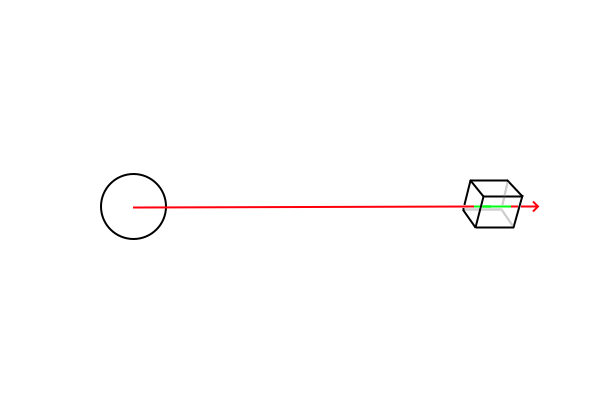
\includegraphics[width = 7 in]{AABB.png}
  \caption{
This figure shows an axis-aligned bounding box and an isotropic emitter, looking from slightly above.
An example field line (red) and intersecting line segment (green) are given.
The bounding box is filled with these intersecting line segments.
It is the gradient of the density of these line segments that forms the gravitational acceleration.
}
\end{figure}

The whole code for this section can be obtained at:

\url{https://github.com/sjhalayka/ellipsoid_emitter}

The following code snippets show how the whole code calculates the gravitational field lines based on a disk-like emitter.
\begin{lstlisting}
bool intersect_AABB(
	const vector_3 min_location, 
	const vector_3 max_location, 
	const vector_3 ray_origin, 
	const vector_3 ray_dir, 
	double &tmin, double &tmax)
{
	 tmin = (min_location.x - ray_origin.x) / ray_dir.x;
	 tmax = (max_location.x - ray_origin.x) / ray_dir.x;

	if (tmin > tmax) swap(tmin, tmax);

	double tymin = (min_location.y - ray_origin.y) / ray_dir.y;
	double tymax = (max_location.y - ray_origin.y) / ray_dir.y;

	if (tymin > tymax) swap(tymin, tymax);
	if ((tmin > tymax) || (tymin > tmax)) return false;
	if (tymin > tmin) tmin = tymin;
	if (tymax < tmax) tmax = tymax;

	double tzmin = (min_location.z - ray_origin.z) / ray_dir.z;
	double tzmax = (max_location.z - ray_origin.z) / ray_dir.z;

	if (tzmin > tzmax) swap(tzmin, tzmax);
	if ((tmin > tzmax) || (tzmin > tmax)) return false;
	if (tzmin > tmin) tmin = tzmin;
	if (tzmax < tmax) tmax = tzmax;

	return true;
}


vector_4 RayEllipsoid(vector_3 ro, vector_3 rd, vector_3 r)
{
	vector_3 r2 = r * r;
	double a = rd.dot(rd / r2);
	double b = ro.dot(rd / r2);
	double c = ro.dot(ro / r2);
	double h = b * b - a * (c - 1.0);

	if (h < 0.0)
		return vector_4(-1, 0, 0, 0);

	double t = (-b - sqrt(h)) / a;

	vector_3 pos = ro + rd * t;

	return vector_4(t, pos.x, pos.y, pos.z);
}

vector_3 EllipsoidNormal(vector_3 pos, vector_3 ra)
{
	vector_3 normal = (pos / (ra * ra));
	normal.normalize();

	return -normal;
}

...

for (size_t i = 0; i < n; i++)
{
	// Something much smaller than unit vectors
	vector_3 oscillator = 
		RandomUnitVector() * 0.01; 

	const vector_4 rv = 
		RayEllipsoid(
			vector_3(0, 0, 0), 
			oscillator, 
			vector_3(1.0 - disk_like, 1.0, 1.0 - disk_like));

	normals[i] = 
		EllipsoidNormal(
			vector_3(rv.y, rv.z, rv.w), 
			vector_3(1.0 - disk_like, 1.0, 1.0 - disk_like));
}

...

for (size_t i = 0; i < n; i++)
{
	vector_3 ray_origin = vector_3(0, 0, 0);
	vector_3 ray_dir = normals[i];

	double tmin = 0, tmax = 0;

	if (intersect_AABB(
		min_location, 
		max_location, 
		ray_origin, 
		ray_dir, 
		tmin, tmax))
	{
		// If pointing in the wrong direction
		if (tmin < 0 || tmax < 0)
			continue;

		vector_3 ray_hit_start = ray_origin + ray_dir * tmin;
		vector_3 ray_hit_end = ray_origin + ray_dir * tmax;

		double intersecting_line_segment_length = 
			(ray_hit_end - ray_hit_start).length();

		density0 += intersecting_line_segment_length;
	}
}

density0 /= 
	(max_location.x - min_location.x) * 
	(max_location.y - min_location.y) * 
	(max_location.z - min_location.z);

...
\end{lstlisting}

See Figs 2, 3, and 4 for visualization of the gravitational field where $D = 3$, $D = 2.1$, and $D = 2.001$.

\begin{figure} 
\centering
\label{fig2}
  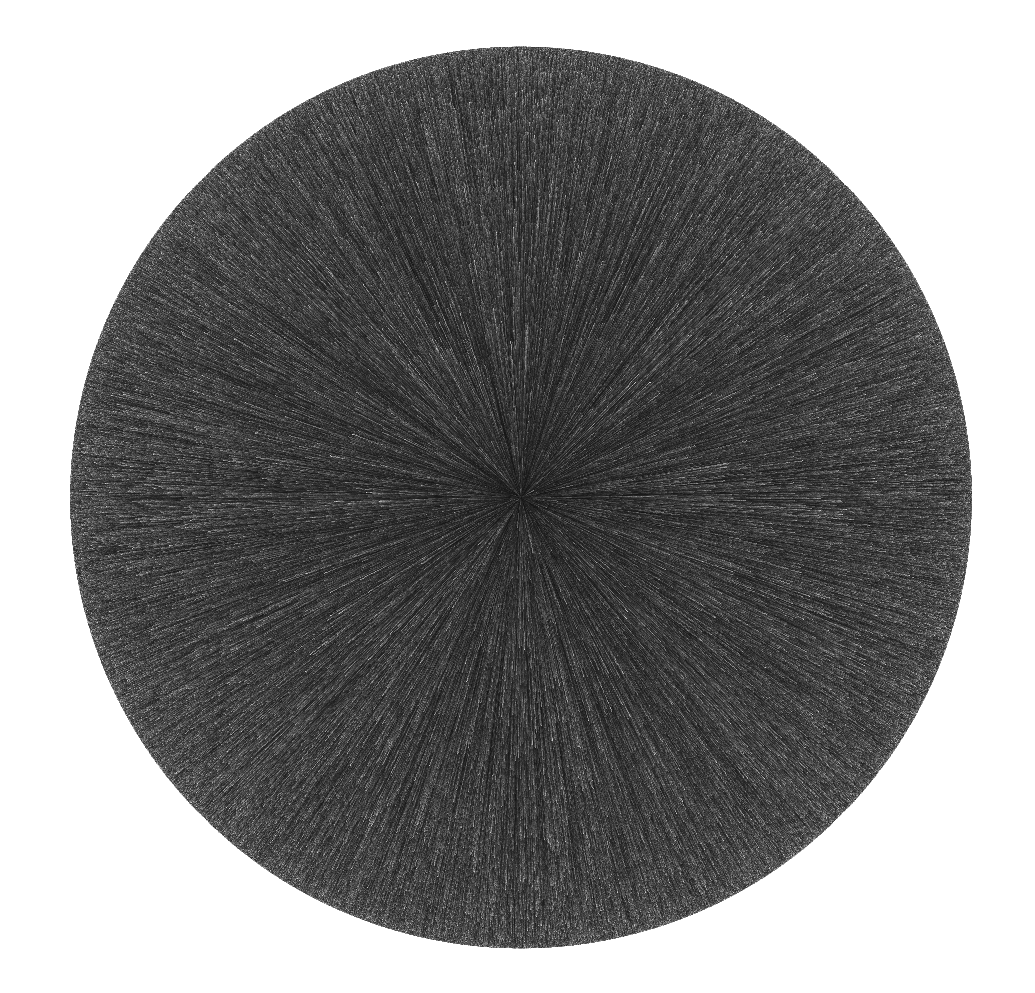
\includegraphics[width = 3 in]{3.png}
  \caption{
Where $D = 3$, as viewed from the side.
The field lines are isotropic, spherical.
}
\end{figure}

\begin{figure} 
\centering
\label{fig3}
  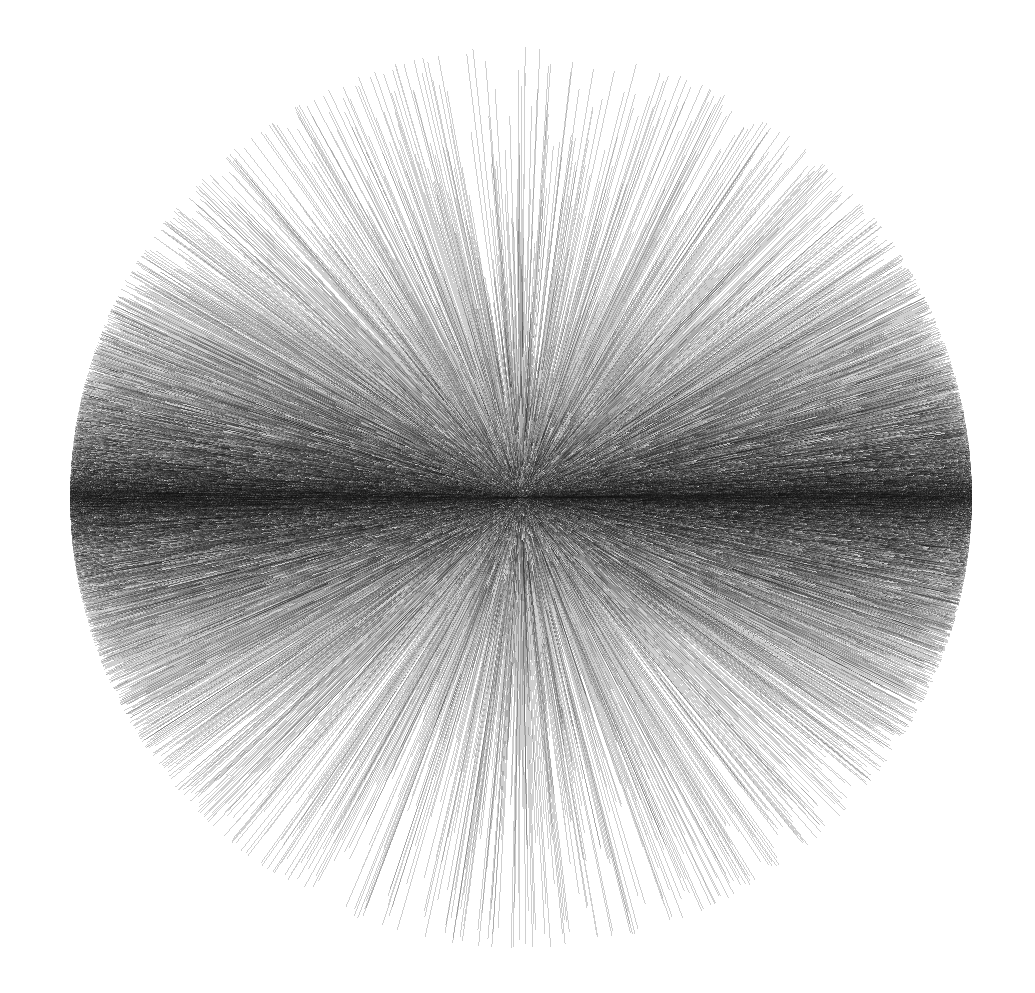
\includegraphics[width = 3 in]{2.1.png}
  \caption{
Where $D = 2.1$, as viewed from the side.
The field lines are increasingly anisotropic.
}
\end{figure}

\begin{figure} 
\centering
\label{fig4}
  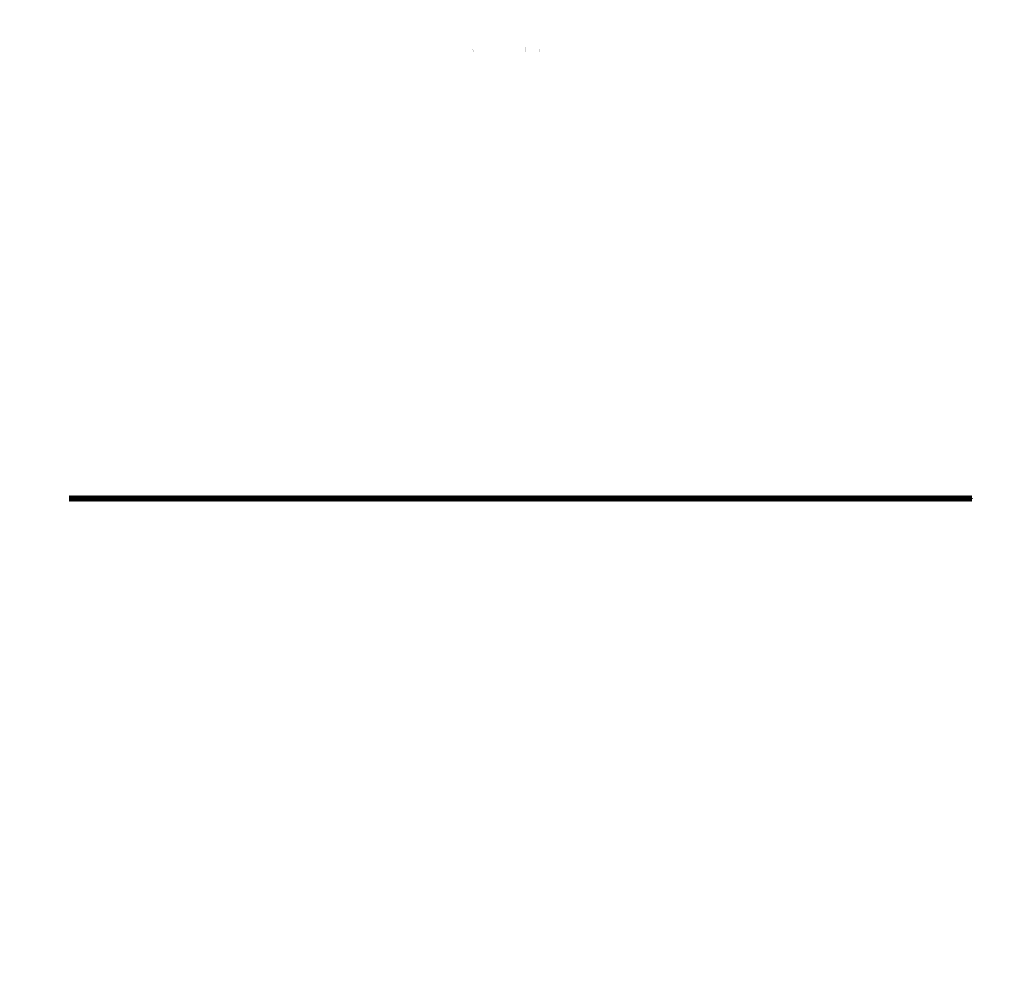
\includegraphics[width = 3 in]{2.001.png}
  \caption{
Where $D = 2.001$, as viewed from the side.
The field lines are anisotropic, disk-like.
}
\end{figure}





\section{Heuristic: field line intersection density gradient}

Below is an analytical code that calculates the dimension $D$ for the Galactic orbit of the Solar System at a speed of $v = 220000$ metres per second.
The output dimension is $D = 2.98352$.
That is, the Galactic gravitational field shape at $R$ is slightly flattened, as observed.
\begin{lstlisting}
#include <cmath>
#include <iostream>
using namespace std;

const double G = 6.67430e-11;
const double c = 299792458;
const double c2 = c * c;
const double c3 = c * c * c;
const double pi = 4.0 * atan(1.0);
const double h = 6.62607015e-34;
const double hbar = h / (2.0 * pi);
const double k = 1.380649e-23;

int main(void)
{
	double M = 1e41;

	double r_s = 2 * G * M / c2;
	double A_s = 4 * pi * r_s * r_s;
	double n = A_s * k * c3 / (4 * G * hbar * log(2.0));

	double R = 3e20;

//	double g = n / (2 * R * R * R);

	double a_Newton = 
		sqrt((n * G * c * hbar * log(2.0)) / 
		(4 * k * pi * R * R * R * R));

//	double a_Newton2 = G * M / (R * R);

	double a_flat = pow(220000, 2.0) / R;

	double v_Newton = sqrt(a_Newton * R);
	double v_flat = 220000;

	double D_final = 3.0 - log(a_flat / a_Newton) / log(R);

	cout << D_final << endl;

	return 0;
}
\end{lstlisting}



\section{Application: visualizing the relativistic Doppler effect}
For the sake of reference, attached here is a visualization that highlights the difference between Newtonian (e.g. Keplerian) orbit and flat rotation curve orbit, in terms of the relativistic Doppler effect.
\begin{figure} 
\centering
\label{fig2}
  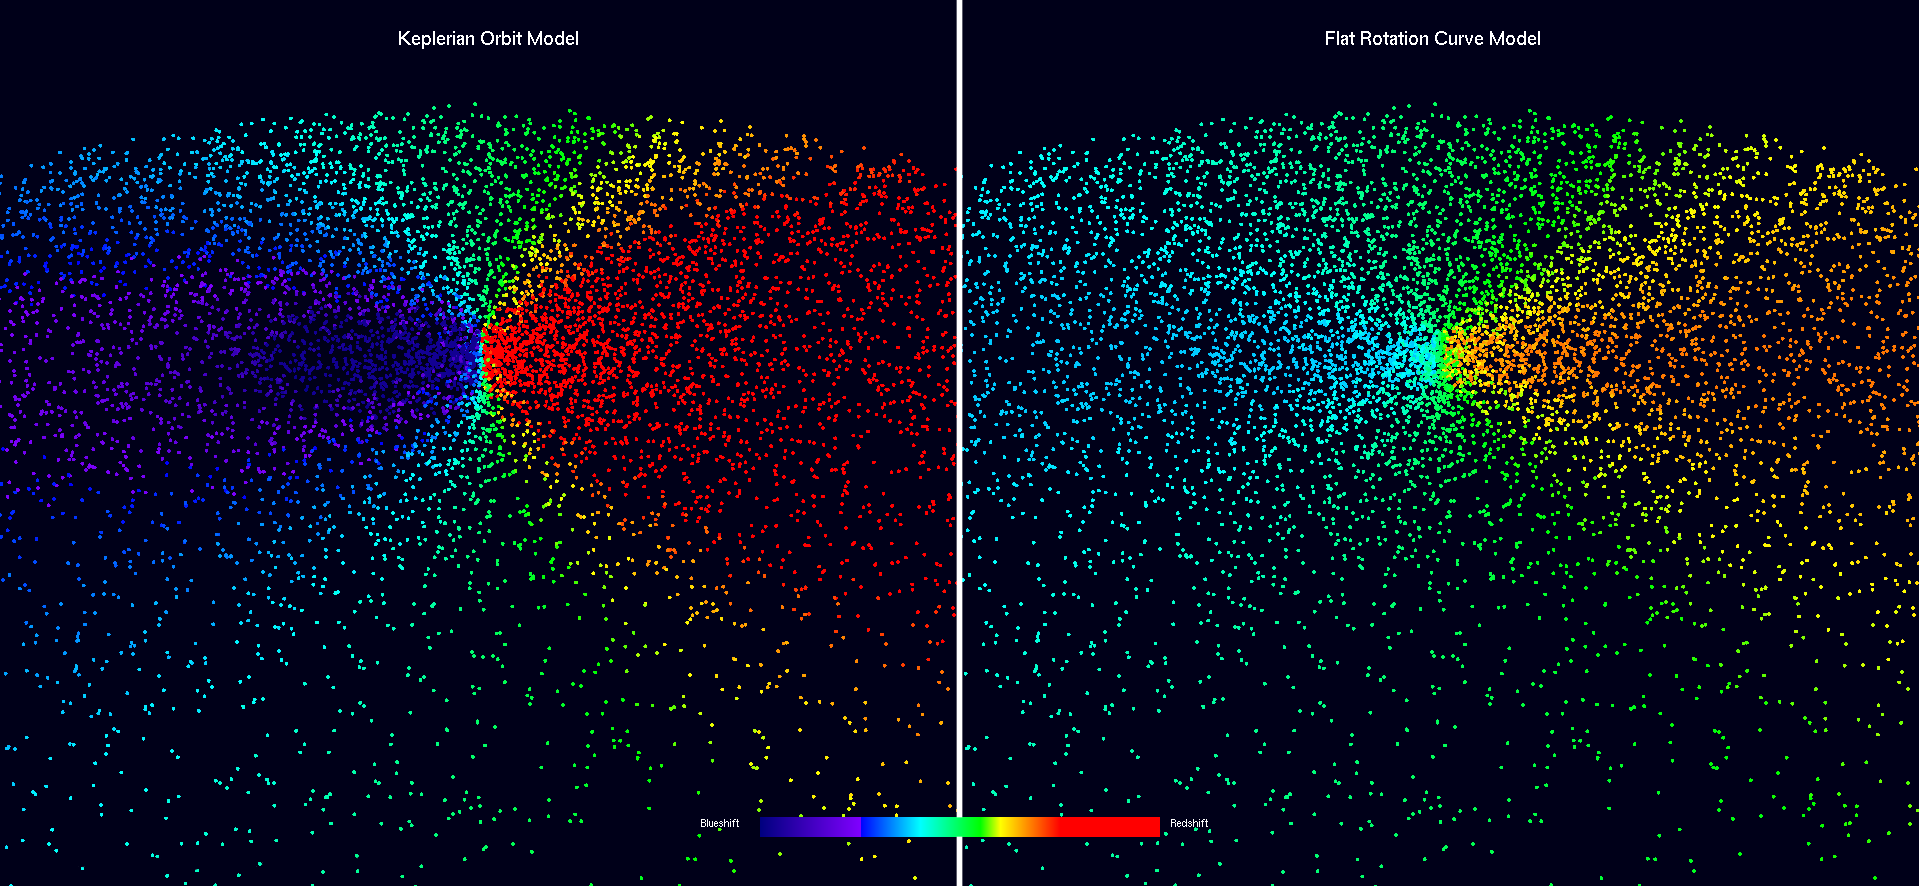
\includegraphics[width = 7 in]{doppler.png}
  \caption{
Visualization of the relativistic Doppler effect for $10^6$ stars.
The Newtonian (e.g. Keplerian) orbit is on the left, and the flat rotation curve orbit is on the right.
}
\end{figure}




\section{Review}

How many bits $n$ does it take to encode $W$ equiprobable microstates?
The answer is: $n = \frac{\log W}{\log 2}$.
For instance, consider a fair $W = 2^n$-sided die, where all sides are equiprobable, and so $p_i = 1/W$.

Both the brute force and heuristic methods for solving the equations are now known for the Newtonian (e.g., Keplerian) orbit, and the Galactic flat rotation curve orbit.

The dimension of the gravitational field is now seen to be fractal.

The relativistic Doppler effect is used to calculate the orbit speed of stars.



\begin{thebibliography}{9}

\bibitem{misner} Misner et al. Gravitation. (1970)

\bibitem{hooft} `t Hooft. Dimensional reduction in quantum gravity. (1993)
\bibitem{susskind} Susskind. The World as a Hologram. (1994)

\bibitem{Mandelbrot} Mandelbrot. How Long Is the Coast of Britain? Statistical Self-Similarity and Fractional Dimension. (1967)


%\bibitem{nasa} Williams. NASA Mercury Fact Sheet. (2024)



\end{thebibliography}









\end{document}









